\documentclass[a4paper, 12pt]{article}
\usepackage[T1]{fontenc}
\usepackage[utf8]{inputenc}

\usepackage{amsmath}
\usepackage{amsfonts}
\usepackage{amssymb}
\usepackage{stmaryrd}
\usepackage[margin=1in]{geometry}
\usepackage[shortlabels]{enumitem}
\usepackage{tikz}

\newcounter{exercise}[section]
\newenvironment{exercise}[1]{\refstepcounter{exercise}\par\medskip
\noindent \textbf{Exercise~\theexercise.} \rmfamily #1
\par\medskip\noindent \textbf{Solution.} \rmfamily}{}
\newcommand{\alternativeSolution}{\par\medskip\noindent \textbf{Solution (alternative).} \rmfamily}

\newcommand{\id}{\operatorname{id}}
\newcommand{\defeq}{\overset{\text{\tiny def}}{=}}
\newcommand{\gfp}{\operatorname{gfp}}
\newcommand{\lfp}{\operatorname{lfp}}
\newcommand{\pre}{\operatorname{pre}}
\newcommand{\post}{\operatorname{post}}
\newcommand{\dotleq}{\mathrel{\dot{\leq}}}
\newcommand{\dotalpha}{\dot{\alpha}}
\newcommand{\dotgamma}{\dot{\gamma}}
\newcommand{\Z}{\mathbb{Z}}
\newcommand{\Bsharp}[1]{\mathcal{B}^\sharp \llbracket #1 \rrbracket}
\newcommand{\Asharp}[1]{\mathcal{A}^\sharp \llbracket #1 \rrbracket}

\title{Software Verification Exercises - Part 2}
\author{Stevanato Giacomo}
\date{06/01/2023}

\begin{document}
    \maketitle

    \begin{exercise}{
    Let $C$ and $A$ be complete lattices and let $(\alpha, C, A, \gamma)$ be a Galois connection. Prove the following properties:
    \begin{enumerate}[(1)]
        \item for any $c_1, c_2 \in C, \gamma(\alpha(c_1 \vee_C c_2)) = \gamma(\alpha(\gamma(\alpha(c_1)) \vee_C \gamma(\alpha(c_2))))$
        \item for all $S \subseteq A, \gamma(\wedge_A S) = \wedge_C \left\{\gamma(a) \in C \mid a \in S \right\}$
        \item $\gamma$ is injective if and only if $\alpha \circ \gamma = \id$ if and only if $\alpha$ is surjective.
    \end{enumerate}
}
    \begin{enumerate}[(1)]
        \item We prove the two directions:
        \begin{itemize}
            \item $(\leq)$:
            \begin{gather*}
                c_i \leq \gamma(\alpha(c_i)) \leq \gamma(\alpha(c_1)) \vee_C \gamma(\alpha(c_2)) \quad\quad \forall i \in \left\{ 1, 2 \right\} \\
                \implies c_1 \vee_C c_2 \leq \gamma(\alpha(c_1)) \vee_C \gamma(\alpha(c_2)) \\
                \implies \gamma(\alpha(c_1 \vee_C c_2)) \leq \gamma(\alpha(\gamma(\alpha(c_1)) \vee_C \gamma(\alpha(c_2))))
            \end{gather*}
            \item $(\geq)$:
            \begin{gather*}
                c_i \leq c_1 \vee_C c_2 \quad\quad \forall i \in \left\{ 1, 2 \right\} \\
                \implies \gamma(\alpha(c_i)) \leq \gamma(\alpha(c_1 \vee_C c_2)) \quad\quad \forall i \in \left\{ 1, 2 \right\} \\
                \implies \gamma(\alpha(c_1)) \vee_C \gamma(\alpha(c_2)) \leq \gamma(\alpha(c_1 \vee_C c_2)) \\
                \implies \alpha(\gamma(\alpha(c_1)) \vee_C \gamma(\alpha(c_2))) \leq \alpha(c_1 \vee_C c_2) \\
                \implies \gamma(\alpha(\gamma(\alpha(c_1)) \vee_C \gamma(\alpha(c_2)))) \leq \gamma(\alpha(c_1 \vee_C c_2))
            \end{gather*}
        \end{itemize}
        \item We prove the two directions:
        \begin{itemize}
            \item $(\leq)$:
            \begin{gather*}
                \wedge_A S \leq a \quad \forall a \in S \\
                \implies \gamma(\wedge_A S) \leq \gamma(a) \quad \forall a \in S \\
                \implies \gamma(\wedge_A S) \leq \wedge_C \left\{\gamma(a) \in C \mid a \in S\right\}
            \end{gather*}
            \item $(\geq)$:
            \begin{gather*}
                \wedge_C \left\{\gamma(a) \in C \mid a \in S\right\} \leq \gamma(a) \quad \forall a \in S \\
                \implies \alpha(\wedge_C \left\{\gamma(a) \in C \mid a \in S\right\}) \leq a \quad \forall a \in S \\
                \implies \alpha(\wedge_C \left\{\gamma(a) \in C \mid a \in S\right\}) \leq \wedge_A S \\
                \implies \wedge_C \left\{\gamma(a) \in C \mid a \in S\right\} \leq \gamma(\wedge_A S)
            \end{gather*}
        \end{itemize}
        \item This is the definition of a Galois Insertion. We prove this by proving the following:
        \begin{itemize}
            \item $\gamma$ is injective $\implies \alpha \circ \gamma = \id$
            \begin{gather*}
                \gamma(a) \leq \gamma(\alpha(\gamma(a))) \\
                \alpha(\gamma(a)) \leq a
                \implies \gamma(\alpha(\gamma(a))) \leq \gamma(a) \\
                \implies \gamma(a) = \gamma(\alpha(\gamma(a))) \\
                \iff a = \alpha(\gamma(a))
            \end{gather*}
            \item $\alpha \circ \gamma = \id \implies \alpha$ is surjective
            \begin{gather*}
                \forall a \in A.\ \alpha(\gamma(a)) = a \\
                \implies \forall a \in A.\ \exists c = \gamma(a) \in C.\ \alpha(c) = a \\
                \implies \alpha \text{ is surjective}
            \end{gather*}
            \item $\alpha$ surjective $\implies \gamma$ injective
            \begin{gather*}
                \alpha(\gamma(\alpha(c))) \leq \alpha(c) \\
                c \leq \gamma(\alpha(c))
                \implies \alpha(c) \leq \alpha(\gamma(\alpha(c))) \\
                \implies \alpha(c) = \alpha(\gamma(\alpha(c))) \\
                \alpha \text{ surjective } \implies \forall a \in A.\ \exists c \in C.\ \alpha(c) = a \\
                \forall a_1, a_2 \in A.\ \gamma(a_1) = \gamma(a_2) \implies \\
                a_1 = \alpha(c_1) = \alpha(\gamma(\alpha(c_1))) = \alpha(\gamma(a_1)) = \alpha(\gamma(a_2)) = \alpha(\gamma(\alpha(c_2))) = \alpha(c_2) = a_2
            \end{gather*}
        \end{itemize}
    \end{enumerate}
\end{exercise}
\clearpage
    \begin{exercise}{
    Let $(\alpha, \left<\wp(State), \subseteq\right>, \left<A, \leq\right>, \gamma)$ be a Galois insertion such that $\left<A, \leq\right>$ is a complete lattice and $\gamma(\bot_A) = \varnothing$. Let us consider a Boolean state predicate $b \in \wp(State)$ and its negation $\neg b \defeq State \setminus b$. Assume that the following conditions hold:
    \begin{enumerate}[(i)]
        \item for all $X \in \wp(State), \alpha(X \cap b) = \alpha(\gamma(\alpha(X)) \cap b)$
        \item for all $X \in \wp(State), \alpha(X \cap \neg b) = \alpha(\gamma(\alpha(X)) \cap \neg b)$
    \end{enumerate}
    Prove that $\gamma(\alpha(b)) = b$ and $\gamma(\alpha(\neg b)) = \neg b$ hold.
}
    \begin{gather*}
        \alpha(b \cap \neg b) = \alpha(\gamma(\alpha(b)) \cap \neg b) = \alpha(\varnothing) \\
        \gamma(\bot_A) = \varnothing \implies \alpha(\varnothing) \leq \bot_A \implies \alpha(\varnothing) = \bot_A \\
        \alpha(\gamma(\alpha(b)) \cap \neg b) = \bot_A \\
        \implies \gamma(\alpha(b)) \cap \neg b \subseteq \gamma(\bot_A) = \varnothing \\
        \implies \gamma(\alpha(b)) \cap \neg b = \gamma(\alpha(b)) \setminus b = \varnothing \\
        \implies \gamma(\alpha(b)) \subseteq b \\
        \implies \gamma(\alpha(b)) = b
    \end{gather*}
    Since $b = \neg \neg b$ by the same argument $\gamma(\alpha(\neg b)) = \neg b$. \\
    The proof didn't use the fact that we were given a Galois insertion.
\end{exercise}
\clearpage
    \begin{exercise}{
    Let $C$ and $A$ be complete lattices, $(\alpha, C, A, \gamma)$ be a Galois insertion, $f: C \to C$ be a monotone concrete operation and $f^\sharp: A \to A$ be a monotone abstract operation. Assume $f \circ \gamma = \gamma \circ f^\sharp$ holds (in this case, $f^\sharp$ is called a $\gamma$-complete approximation of $f$).
    \begin{enumerate}[1.]
        \item Prove that $\alpha(\gfp(f)) = \gfp(f^\sharp)$
        \item Give a counterexample to the equality $\alpha(\lfp(f)) = \lfp(f^\sharp)$
    \end{enumerate}
}
    \begin{enumerate}[1.]
        \item We prove the two directions:
        \begin{itemize}
            \item $(\geq)$
            \begin{gather*}
                \gamma(\gfp(f^\sharp)) = \gamma(f^\sharp (\gfp(f^\sharp))) = f(\gamma(\gfp(f^\sharp))) \\
                \implies \gamma(\gfp(f^\sharp)) \leq \gfp(f) \\
                \gfp(f^\sharp) = \alpha(\gamma(\gfp(f^\sharp))) \leq \alpha(\gfp(f))
            \end{gather*}
            \item $(\leq)$
            \begin{gather*}
                \begin{aligned}
                    \alpha(\gfp(f)) &= \alpha(f(\gfp(f))) \\
                    &\leq \alpha(f(\gamma(\alpha(\gfp(f))))) \\
                    &= \alpha(\gamma(f^\sharp(\alpha(\gfp(f))))) \\
                    &= f^\sharp(\alpha(\gfp(f)))
                \end{aligned} \\
                \implies \alpha(\gfp(f)) \leq \gfp(f^\sharp)
            \end{gather*}
            (Fixpoint induction lemma for greatest fixpoint, without requirement of $f$ being continuous but only monotone)
        \end{itemize}
        \item Consider for example $C = \{0, 1, 2\}$, $A = \{x, y\}$ with a linear order. They are clearly lattices. $\alpha$ and $\gamma$ as defined as the following:
        \begin{gather*}
            \begin{aligned}
                \alpha(0) = x \\
                \alpha(1) = x \\
                \alpha(2) = y
            \end{aligned}
            \qquad\qquad
            \begin{aligned}
                \gamma(x) = 1 \\
                \gamma(y) = 2
            \end{aligned}
        \end{gather*}
        This is a Galois insertion, in fact:
        \begin{gather*}
            \begin{aligned}
                0 \leq \gamma(\alpha(0)) = \alpha(x) = 1 \\
                1 \leq \gamma(\alpha(1)) = \alpha(x) = 1 \\
                2 \leq \gamma(\alpha(2)) = \alpha(y) = 2
            \end{aligned}
            \qquad\qquad
            \begin{aligned}
                \alpha(\gamma(x)) = \alpha(1) = x \\
                \alpha(\gamma(y)) = \alpha(2) = y
            \end{aligned}
        \end{gather*}
        Consider the following $f$ and the induced $f^\sharp = \alpha \circ f \circ \gamma$ by $\gamma \circ f^\sharp = f \circ \gamma$:
        \begin{gather*}
            \begin{aligned}
                f(0) = 0 \\
                f(1) = 2 \\
                f(2) = 2
            \end{aligned}
            \qquad\quad
            \begin{aligned}
                f^\sharp (x) = y \\
                f^\sharp (y) = y
            \end{aligned}
            \qquad\quad
            \begin{aligned}
                \gamma(f^\sharp(x)) = \gamma(y) = 2 = f(1) = f(\gamma(x)) \\
                \gamma(f^\sharp(y)) = \gamma(y) = 2 = f(2) = f(\gamma(y)) \\
            \end{aligned}
        \end{gather*}
        $0$ and $2$ are fixpoints of $f$, thus $\lfp(f) = 0$. $y$ is the only fixpoint of $f^\sharp$, so $\lfp(f^\sharp) = y$. However $\alpha(\lfp(f)) = \alpha(0) = x \neq y = \lfp(f^\sharp)$.
    \end{enumerate}
\end{exercise}
\clearpage
    \begin{exercise}{
    Let $C$ and $A$ be complete lattices, $(\alpha, C, A, \gamma)$ be a Galois insertion, $f: C \to C$ be a monotone function. Prove that $\gamma(\lfp(\alpha \circ f \circ \gamma)) = \lfp(\gamma \circ \alpha \circ f)$
}
    We prove the two directions:
    \begin{itemize}
        \item $\leq$
        \begin{gather*}
            \begin{aligned}
                (\alpha \circ f)(\lfp(\gamma \circ \alpha \circ f))
                &= (\alpha \circ f \circ \gamma \circ \alpha \circ f)(\lfp(\gamma \circ \alpha \circ f)) \\
                &= (\alpha \circ f \circ \gamma)((\alpha \circ f)(\lfp(\gamma \circ \alpha \circ f)))
            \end{aligned} \\
            \implies \lfp(\alpha \circ f \circ \gamma) \leq (\alpha \circ f)(\lfp(\gamma \circ \alpha \circ f)) \\
            \implies \gamma(\lfp(\alpha \circ f \circ \gamma)) \leq (\gamma \circ \alpha \circ f)(\lfp(\gamma \circ \alpha \circ f)) = \lfp(\gamma \circ \alpha \circ f)
        \end{gather*}
        \item $\geq$
        \begin{gather*}
            \begin{aligned}
                \gamma(\lfp(\alpha \circ f \circ \gamma))
                &= (\gamma \circ \alpha \circ f \circ \gamma) (\lfp(\alpha \circ f \circ \gamma)) \\
                &= (\gamma \circ \alpha \circ f)(\gamma(\lfp(\alpha \circ f \circ \gamma)))
            \end{aligned} \\
            \implies \lfp(\gamma \circ \alpha \circ f) \leq \gamma(\lfp(\alpha \circ f \circ \gamma))
        \end{gather*}
    \end{itemize}
\end{exercise}
\clearpage
    \begin{exercise}{
    Let $R \subseteq S \times S$ be a binary relation on a set $S$. Let us define the following functions of type $\wp(S) \to \wp(S)$.
    \begin{itemize}
        \item $\pre_R \defeq \lambda Y. \left\{ x \in S \mid \exists y \in Y.\ (x, y) \in R \right\}$
        \item $\widetilde{\pre}_R \defeq \lambda Y. \left\{ x \in S \mid \forall y \in S.\ ((x, y) \in R \implies y \in Y)\right\}$
        \item $\post_R \defeq \lambda X. \left\{ y \in S \mid \exists x \in X.\ (x, y) \in R \right\}$
        \item $\widetilde{\post}_R \defeq \lambda X. \left\{ y \in S \mid \forall x \in S.\ ((x, y) \in R \implies x \in X)\right\}$
    \end{itemize}
    Prove that $(\pre_R, \left<\wp(S), \subseteq\right>, \left<\wp(S), \subseteq\right>, \post_R)$ and $(\post_R, \left<\wp(S), \subseteq\right>, \left<\wp(S), \subseteq\right>, \pre_R)$ are both Galois connections.
}
    TODO
\end{exercise}
\clearpage
    \begin{exercise}{
    Let $(\alpha_1, C_1, A_1, \gamma_1)$ and $(\alpha_2, C_2, A_2, \gamma_2)$ be Galois connections where $C_i$ and $A_i$ ($i = 1,2$) are complete lattices. Let $\left<C_1 \to^m C_2, \sqsubseteq\right>$ and $\left<A_1 \to^m A_2, \sqsubseteq\right>$ denote the complete lattices of monotone functions ordered with the pointwise ordering: $f \sqsubseteq g$ iff $\forall x.\ f(x) \leq g(x)$. Define $\alpha : (C_1 \to^m C_2) \to (A_1 \to^m A_2)$ by $\alpha(f) \defeq \alpha_2 \circ f \circ \gamma_1$ and $\gamma: (A_1 \to^m A_2) \to (C_1 \to^m C_2)$ by $\gamma(f^\sharp) \defeq \gamma_2 \circ f^\sharp \circ \alpha_1$. \\
    Prove that $(\alpha, C_1 \to^m C_2, A_1 \to^m A_2, \gamma)$ is a Galois connection.
}
    \begin{enumerate}[1.]
        \item $\left<C_1 \to^m C_2, \sqsubseteq\right>$ and $\left<A_1 \to^m A_2, \sqsubseteq\right>$ are lattices by hypothesis.
        \item $\alpha$ monotone ($\forall f_1, f_2 \in C_1 \to^m C_2.\ f_1 \sqsubseteq f_2 \implies \alpha(f_1) \sqsubseteq \alpha(f_2)$):
        \begin{gather*}
            f_1 \sqsubseteq f_2 \implies \forall c \in C_1.\ f_1 (c) \leq f_2 (c) \\
            \implies f_1 (\gamma_1 (a)) \leq f_2 (\gamma_1 (a)) \qquad \forall a \in A_1 \\
            \implies \alpha_2 (f_1 (\gamma_1 (a))) \leq \alpha_2 (f_2 (\gamma_1 (a))) \\
            \implies \alpha(f_1)(a) \leq \alpha(f_2)(a) \\
            \implies \alpha(f_1) \subseteq \alpha(f_2)
        \end{gather*}
        \item $\gamma$ monotone ($\forall f^\sharp_1, f^\sharp_2 \in A_1 \to^m A_2.\ f^\sharp_1 \sqsubseteq f^\sharp_2 \implies \gamma(f^\sharp_1) \sqsubseteq \gamma(f^\sharp_2)$):
        \begin{gather*}
            f^\sharp_1 \sqsubseteq f^\sharp_2 \implies \forall a \in A_1.\ f^\sharp_1 (a) \leq f^\sharp_2 (a) \\
            \implies f^\sharp_1 (\alpha_1 (c)) \leq f^\sharp_2 (\alpha_1 (c)) \qquad \forall c \in C_1  \\
            \implies \gamma_2 (f^\sharp_1 (\alpha_1 (c))) \leq \gamma_2 (f^\sharp_2 (\alpha_1 (c))) \\
            \implies \gamma(f^\sharp_1)(c) \leq \gamma(f^\sharp_2)(c) \\
            \implies \gamma(f^\sharp_1) \subseteq \gamma(f^\sharp_2)
        \end{gather*}
        \item $\forall f \in C_1 \to^m C_2.\ f \sqsubseteq \gamma(\alpha(f))$:
        \begin{gather*}
            c \leq \gamma_1 (\alpha_1 (c)) \qquad \forall c \in C_1 \\
            \implies f(c) \leq f(\gamma_1 (\alpha_1 (c))) \\
            \implies f(c) \leq \gamma_2(\alpha_2(f(c))) \leq \gamma_2(\alpha_2(f(\gamma_1 (\alpha_1 (c))))) \\
            \implies f \sqsubseteq \gamma(\alpha(f))
        \end{gather*}
        \item $\forall f^\sharp \in A_1 \to^m A_2.\ \alpha(\gamma(f^\sharp)) \sqsubseteq f^\sharp$:
        \begin{gather*}
            \alpha_1(\gamma_1(c)) \leq c \qquad \forall c \in C_1 \\
            \implies f^\sharp(\alpha_1(\gamma_1(c))) \leq f^\sharp(c) \\
            \implies \alpha_2(\gamma_2(f^\sharp(\alpha_1(\gamma_1(c))))) \leq \alpha_2(\gamma_2(f^\sharp(c))) \leq f^\sharp(c) \\
            \implies \alpha(\gamma(f^\sharp)) \sqsubseteq f^\sharp
        \end{gather*}
    \end{enumerate}
\end{exercise}
\clearpage
    \begin{exercise}{
    Let $S$ be any set, $\left<L, \leq\right>$ be a complete lattice and consider $L^S \triangleq S \to L$ endowed with the following pointwise order relation $\dotleq$ between functions: $f_1 \dotleq f_2$ when for all $x \in S$, $f_1(x) \leq f_2(x)$. \\
    Let $(\alpha, \left<C, \leq_C\right>, \left<A, \leq_A\right>, \gamma)$ be a Galois connection. Prove that $(\dotalpha, C^S, A^S, \dotgamma)$ is a Galois connection, where:
    \begin{itemize}
        \item $\dotalpha(f) \triangleq \lambda x.\ \alpha(f(x))$
        \item $\dotgamma(g) \triangleq \lambda x.\ \gamma(g(x))$
    \end{itemize}
}
    \begin{enumerate}[1.]
        \item $C^S$ and $A^S$ are posets by hypothesis.
        \item $\dotalpha$ is monotonic ($\forall f_1, f_2 \in C^S.\ f_1 \dotleq f_2 \implies \dotalpha(f_1) \dotleq \dotalpha(f_2))$
        \begin{gather*}
            f_1 \dotleq f_2 \implies \forall x \in S.\ f_1(x) \leq_C f_2(x) \\
            \implies \alpha(f_1(x)) \leq_A \alpha(f_2(x)) \\
            \implies \dotalpha(f_1)(x) \leq_A \dotalpha(f_2)(x) \\
            \implies \dotalpha(f_1) \dotleq \dotalpha(f_2)
        \end{gather*}
        \item $\dotgamma$ is monotonic ($\forall g_1, g_2 \in A^S.\ g_1 \dotleq g_2 \implies \dotgamma(g_1) \dotleq \dotgamma(g_2))$
        \begin{gather*}
            g_1 \dotleq g_2 \implies \forall x \in S.\ g_1(x) \leq_A g_2(x) \\
            \implies \gamma(g_1(x)) \leq_C \gamma(g_2(x)) \\
            \implies \dotgamma(g_1)(a) \leq_C \dotgamma(g_2)(a) \\
            \implies \dotgamma(g_1) \dotleq \dotgamma(g_2)
        \end{gather*}
        \item $\forall f \in C^S.\ f \dotleq \dotgamma(\dotalpha(f))$
        \begin{gather*}
            c \leq_C \gamma(\alpha(c)) \quad \forall c \in C \\
            \implies f(x) \leq_C \gamma(\alpha(f(x))) \quad \forall x \in S \\
            \implies f(x) \leq_C \dotgamma(\dotalpha(f))(x) \\
            \implies f \dotleq \dotgamma(\dotalpha(f))
        \end{gather*}
        \item $\forall g \in A^S.\ \dotalpha(\dotgamma(g)) \dotleq g$
        \begin{gather*}
            \alpha(\gamma(a)) \leq_A a \quad \forall a \in A \\
            \implies \alpha(\gamma(g(x))) \leq_A g(x) \quad \forall x \in S \\
            \implies \dotalpha(\dotgamma(g))(x) \dotleq g(x) \\
            \implies \dotalpha(\dotgamma(g)) \dotleq g
        \end{gather*}
    \end{enumerate}
\end{exercise}
\clearpage
    \begin{exercise}{
    Let $C$ and $A$ be complete lattices, $(\alpha, C, A, \gamma)$ be a Galois insertion, $f: C \to C$ be an additive concrete operation (i.e. for all $S \subseteq C$, $f(\vee_C S) = \vee_C f(S)$). Prove that: there exists a monotone abstract operation $f^\sharp: A \to A$ such that $\alpha \circ f = f^\sharp \circ \alpha$ holds if and only if for all $a \in A$ there exists some $a' \in A$ such that $\vee_C \left\{ c \in C \mid f(c) \leq \gamma(a) \right\} = \gamma(a')$
}
    We prove the two directions:
    \begin{itemize}
        \item $(\implies)$ \\
        Let $S = \{c \in C \mid f(c) \leq \gamma(a)\}$, $c^* = \vee_C S$. Then:
        \begin{gather*}
            \begin{aligned}
                (f \circ \gamma \circ \alpha) (c^*)
                &\leq (\gamma \circ \alpha \circ f \circ \gamma \circ \alpha) (c^*) \\
                &= (\gamma \circ f^\sharp \circ \alpha \circ \gamma \circ \alpha) (c^*) \\
                &= (\gamma \circ f^\sharp \circ \alpha) (c^*) \\
                &= (\gamma \circ \alpha \circ f) (c^*) \\
                &= (\gamma \circ \alpha) (\vee_C \left\{f(c) \mid c \in C, f(c) \leq \gamma(a)\right\}) \\
                % \gamma(a) is an upper bound of f(S) (not necessarily the least)
                &\leq (\gamma \circ \alpha \circ \gamma) (a) \\
                &= \gamma (a)
            \end{aligned} \\
            \implies (\gamma \circ \alpha) (c^*) \in S \\
            \implies (\gamma \circ \alpha) (c^*) \leq c^* \qquad\qquad c^* \leq (\gamma \circ \alpha) (c^*) \\
            \implies (\gamma \circ \alpha) (c^*) = c^* \\
            \implies a' = \alpha(c^*)
        \end{gather*}
        \item $(\impliedby)$ \\
        We want to show $f^\sharp = \alpha \circ f \circ \gamma$ is the wanted function. It is monotone because a composition of monotone function. Then we want to show $\alpha \circ f = f^\sharp \circ \alpha = \alpha \circ f \circ \gamma \circ \alpha$, that is $\forall c \in C.\ (\alpha \circ f)(c) = (\alpha \circ f \circ \gamma \circ \alpha)(c)$ \\
        We distinguish the two directions:
        \begin{itemize}
            \item $(\leq)$
            \begin{gather*}
                c \leq \gamma(\alpha(c)) \\
                \implies (\alpha \circ f)(c) \leq (\alpha \circ f \circ \gamma \circ \alpha)(c)
            \end{gather*}
            \item $(\geq)$ \\
            Let $a = \alpha(f(c))$, $S = \left\{\dot{c} \in C \mid f(\dot{c}) \leq \gamma(a)\right\}$, $c^* = \vee_C S = \gamma(a')$.
            \begin{gather*}
                f(c) \leq \gamma(\alpha(f(c))) \implies c \in S \implies c \leq c^* \\
                \implies \gamma(\alpha(c)) \leq \gamma(\alpha(c^*)) = \gamma(\alpha(\gamma(a'))) = \gamma(a') = c^* \\
                \begin{aligned}
                    \implies \alpha(f(\gamma(\alpha(c))))
                    &\leq \alpha(f(c^*)) \\
                    &= \alpha(f(\vee_C S)) \\
                    &= \alpha(\vee_C \left\{f(\dot{c}) \mid \dot{c} \in C, f(\dot{c}) \leq \gamma(\alpha(f(c)))\right\}) \\
                    % \gamma(\alpha(f(c))) is an upper bound of f(S) (not necessarily the least)
                    &\leq \alpha(\gamma(\alpha(f(c)))) \\
                    &= \alpha(f(c))
                \end{aligned}
            \end{gather*}
        \end{itemize}
    \end{itemize}
    Note: this proof didn't use the properties of a Galois insertion, only $\alpha = \alpha \circ \gamma \circ \alpha$ and $\gamma = \gamma \circ \alpha \circ \gamma$, which are properties of Galois connections too (see exercise 1).
\end{exercise}
\clearpage
    \begin{exercise}{
    Consider the following abstract domain $Sign_k$ of $\left<\wp(\Z), \subseteq\right>$ where $k \in \Z$ is any given integer:
    \begin{center}
        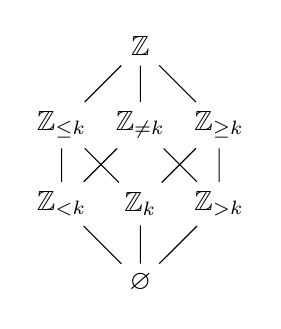
\begin{tikzpicture}
            \node (top) at (1, 3) {$\Z$};
            \node (leq) at (0, 2) {$\Z_{\leq k}$};
            \node (neq) at (1, 2) {$\Z_{\neq k}$};
            \node (geq) at (2, 2) {$\Z_{\geq k}$};
            \node (lt) at (0, 1) {$\Z_{< k}$};
            \node (eq) at (1, 1) {$\Z_{k}$};
            \node (gt) at (2, 1) {$\Z_{> k}$};
            \node (bot) at (1, 0) {$\varnothing$};

            \draw (top) -- (leq) -- (eq);
            \draw (top) -- (neq) -- (lt);
            \draw (top) -- (geq) -- (gt);
            \draw (leq) -- (lt) -- (bot);
            \draw (neq) -- (gt) -- (bot);
            \draw (geq) -- (eq) -- (bot);
        \end{tikzpicture}
    \end{center}
    Hence, $Sign_k$ is a parametric abstract domain of signs, where the constant 0 is replaced by any integer parameter $k \in \Z$. Provide sound definitions for the following abstract transfer functions: $\Bsharp{x \leq k}$, $\Asharp{x * y}$, $\Asharp{x / k}$, $\Asharp{x - y}$, which are as precise as possible, ideally the best correct approximation.
}
    \begin{align*}
        \Bsharp{x \leq k} s^\sharp &= \begin{cases}
            \bot^\sharp & \text{if } \Asharp{x} s^\sharp \in \{ \varnothing, \Z_{>k} \} \text{ or } s^\sharp = \bot^\sharp \\
            s^\sharp [x \to \Z_{\leq k}] & \text{if } \Asharp{x} s^\sharp \in \{ \Z, \Z_{\leq k} \} \\
            s^\sharp [x \to \Z_k] & \text{if } \Asharp{x} s^\sharp \in \{ \Z_k, \Z_{\geq k} \} \\
            s^\sharp [x \to \Z_{< k}] & \text{if } \Asharp{x} s^\sharp \in \{ \Z_{< k}, \Z_{\neq k} \} \\
            ... & \text{(specialized cases for e.g. $x - y \leq k$)}
        \end{cases} \\
        \Asharp{x * y} s^\sharp &= \begin{cases}
            \varnothing & \text{if } \Asharp{x} s^\sharp = \varnothing \text{ or } \Asharp{y} s^\sharp = \varnothing \text{ or } s^\sharp = \bot^\sharp \\
            \Z_k & \text{if } k = 0 \text{ and } (\Asharp{x} = \Z_k \text{ or } \Asharp{y} = \Z_k) \\
            \Asharp{y} s^\sharp \hspace*{-0.3cm} & \text{if } k = 1 \text{ and } \Asharp{x} s^\sharp = \Z_k \\
            \Z_{>k} & \text{if } k > 0, \Asharp{x} s^\sharp \in \{ \Z_k, \Z_{>k}, \Z_{\geq k} \} \text{ and } \Asharp{y} s^\sharp \in \{ \Z_k, \Z_{>k}, \Z_{\geq k} \} \\
            ... & \text{(invert $x$ and $y$)} \\
            \Z & \text{otherwise}
        \end{cases} \\
        \Asharp{x / k} s^\sharp &= \begin{cases}
            \varnothing & \text{if } \Asharp{x} s^\sharp = \varnothing, k = 0 \text{ or } s^\sharp = \bot^\sharp \\
            \Asharp{x} s^\sharp & \text{if } k = 1 \\
            \Z_{< k} & \text{if } k > 1 \text{ and } \Asharp{x} s^\sharp \in \{ \Z_{< k}, \Z_{\leq k} \} \\
            \Z_{> k} & \text{if } k < 0 \text{ and } \Asharp{x} s^\sharp \in \{ \Z_{< k}, \Z_{\leq k} \} \\
            \Z_{\neq k} & \text{if } \Asharp{x} = \Z_k \\
            ... \\
            \Z & \text{otherwise}
        \end{cases} \\
        \Asharp{x - y} s^\sharp &= \begin{cases}
            \varnothing & \text{if } \Asharp{x} s^\sharp = \varnothing, \Asharp{y} s^\sharp = \varnothing \text{ or } s^\sharp = \bot^\sharp \\
            \Asharp{x} s^\sharp \hspace*{-0.3cm} & \text{if } k = 0 \text{ and } \Asharp{y} s^\sharp = \Z_k \\
            \Z_{< k} & \text{if } k > 0, \Asharp{x} s^\sharp \in \{ \Z_{< k}, \Z_{\leq k}, Z_k \} \text{ and } \Asharp{y} s^\sharp \in \{ \Z_{> k}, \Z_{\geq k}, Z_k \} \\
            ... & \text{(invert $x$ and $y$ and negate their values)} \\
            \Z & \text{otherwise}
        \end{cases} \\
    \end{align*}
\end{exercise}
\clearpage
\end{document}
